\documentclass[a4paper,12pt]{article}
 \usepackage{color}
 \usepackage{graphicx}
 \usepackage{csquotes}
 \usepackage[italian]{babel}
 %impostazioni per inserire codice formattato
\usepackage{listings}
\usepackage{color}
\usepackage{pbox}
\definecolor{dkgreen}{rgb}{0,0.6,0}
\definecolor{gray}{rgb}{0.5,0.5,0.5}
\definecolor{mauve}{rgb}{0.58,0,0.82}

\lstset{frame=tb,
  language=Java,
  aboveskip=3mm,
  belowskip=3mm,
  showstringspaces=false,
  columns=flexible,
  basicstyle={\small\ttfamily},
  numbers=none,
  numberstyle=\tiny\color{gray},
  keywordstyle=\color{blue},
  commentstyle=\color{dkgreen},
  stringstyle=\color{mauve},
  breaklines=true,
  breakatwhitespace=true,
  tabsize=3
}
\begin{document}
\title{Progetto Tweb}
\author{Silvestro Stefano Frisullo \\ mat. 832813}
\date{\today}
\maketitle
\pagenumbering{roman}
\tableofcontents

\newpage
\pagenumbering{arabic}

\section{Tema e sezioni del sito}
Il tema del sito è un e-commerce di scarpe.
È possibile scegliere tra diversi modelli, classici o sportivi e per uomo o donna.
Per ogni modello è presente nome, descrizione, taglia disponibile e prezzo.

Le sezioni \textit{commerciali} del sito sono:
\begin{itemize}
	\item Man
	\item Woman
	\item Classic
	\item Sport
	\item Sneakers
\end{itemize}
La parte superiore presenta 4 pulsanti:
\begin{itemize}
	\item Home
	\item Login/Logout
	\item Wishlist
	\item Carrello
\end{itemize}

\section{Funzionalità}
\subsection{Login}
Appena l'utente accede ad una qualsiasi pagina del sito, se non ha una sessione valida attiva,
viene reindirizzato su \textit{login.html}. Questa pagina prevede due opzioni: il login tramite
username e password e la registrazione. L'utente può loggarsi inserendo username e password oppure
essere autenticato dal sistema se in possesso del cookie di login persistente.
I file coinvolti sono: \textit{login.js} e \textit{login.php}. Nel caso di login tradizionale javascript
manda una ajax request al server, il quale farà query sul database, e in caso affermativo
autenticherà l'utente, creerà la sessione e il cookie di login persistente valido 24 ore.
Il cookie è un hash con sha256 di username + timestamp Unix + un numero casuale tra 0 e 100000000
generato con \textit{random\textunderscore int}.
Nel caso di autenticazione con cookie,\textit{login.js} manderà ajax request col contenuto di tale cookie e
se uguale a quello nel database l'utente è accettato.

\subsection{Logout}
Per fettuare il logout, bisogna cliccare suul'icona a forma di utente.
La pagina che gestiste il logout è sempre \textit{login.html}, ma opportunamente modificata dal codice javascript
di \textit{login.js}, in modo da informare l'utente di essere già autenticato tramite un'immagine e la scritta
\textit{Already logged in ;) }. Al logout viene cancellato il cookie persistente di login, quindi bisognerà
reinserire username e password.
\subsection{Registrazione}
Per la registrazione sono coinvolti i file \textit{login.js} e \textit{register.php}.
Javascript manda i campi non vuoti al server che controlla che l'username non sia già
occupato e libero crea il profilo utente. Successivamente l'utente può loggarsi.

\subsection{Gestione del contenuto generato dall'utente}
I contenuti generabili dall'utente sono la \textbf{wishlist} e il \textbf{carrello}.
\subsubsection{Wishlist}
La \textbf{wishlist}, a cui si accede cliccando sull'icona del cuore, è gestita dai file
\textit{wishlist.html}, \textit{wishlist.js}, \textit{wishlist.php}, \textit{add-wishlist.php},
\textit{remove-wishlist.php}. Per scelta progettuale, la wishlist è memorizzata all'interno di una tabella nel database
e non è possibile aggiunge lo stesso oggetto più volte.
Riprendendo lo stile della home, la wishlist permette di visualizzare le scarpe, aggiungerle o rimuoverle.
Javascript manda un'ajax request senza dati  a \textit{wishlist.php},
il quale prenderà da \textdollar\textunderscore SESSION l'id dell'utente.
Con l'id utente fa query e ricava tutte le scarpe, crea gli oggetti
\textit{Shoe} corrispondenti e le restituisce in formato JSON secondo questa sintassi:

\begin{lstlisting}
[{	"id":"3", //id univoco scarpa
	"model":"Classic",
	"price":"200",
	"description":"perfect for classy man",
	"image":"images\/scarpa-classica.jpg" // percorso relativo immagine
	}]
\end{lstlisting}
in caso di successo, javascript rappresenta ogni scarpa in html e inserisce il codice
nel corpo della pagina.
In \textit{wishlist.html}, ogni scheda ha un bottone \textit{Remove},
che tramite  \textit{removeWishlist} manderà una ajax request a \textit{remove-wishlist.php},
con id del prodotto da rimuovere dalla wishlist (quindi ci sono due ID, uno è dell'utente
ed è salvato in \textdollar\textunderscore SESSION, l'altro è della scarpa e si trova in \textdollar\textunderscore GET ).
\textit{remove-wishlist.php} farà una query sul database e rimuoverà dalla wishlist la scarpa con
quell'ID restituendo "ok". A quel punti javascript eliminerà il nodo DOM dell'oggetto
e aggiornerà la pagina.
Per aggiungere un oggetto alla wishlist, si hanno due opzioni: tascinarlo sull'icona del cuore
oppure cliccarci sopra, e in seguito cliccare su "Add to wishlist".
I file che gestiscono questo caso sono \textit{wishlist.js} e \textit{add-wishlist.php}.
Il primo si occupa dell'animazione e delle chiamate ajax, mentre il secondo tramite id della scarpa
fa una query al database. Dato che non è possibile inserire più di una volta lo stesso
oggetto, nel caso in cui sià già presente il server restituisce "duplicate", e l'utente è
notificato che il prodotto è già in wishlist. Altrimenti, se tutto va bene, javascript
rimuove la scheda del prodotto dalla pagina, in modo da dare un feedback visivo
della corretta esecuzione dell'operazione, ma senza essere troppo invadenti.
Stesso funzionament per quando si aggiunge alla wishlist dalla pagina del prodotto
\textit{shop-single.html}, ma in questo caso il file javascript responsabile della ajax request è
\textit{single-item.js}.
\subsubsection{Carrello}
Diversamente dalla \textit{wishlist}, il carrello è implementato tramite variabili di sessione.
Gli oggetti possono essere aggiunti o rimossi, e l'aggiunta come per la wishlist può avvenire trascinando
gli oggetti o cliccando sul bottone relativo.
L'array che contiene i dati del carrello è \textdollar\textunderscore SESSION[ "items"] e i file coinvolti sono
\textit{cart.html}, \textit{cart.js}, \textit{request.js}, \textit{show-single.js}, \textit{cart.php}, \textit{add-cart.php}, \textit{remove-cart.php}.
In fondo alla pagina  è indicato il costo totale degli oggetti nel carrello e il bottone "Buy!" simula una
vendita fittizia, fa comparire un'immagine di conferma all'untente e svuota il carrello.
Cliccare sul bottone Buy con carrello vuoto farà apparire la scritta
\textit{You need to add something to the cart first!}.
Per l'aggiunta al carrello, sia tramite trascinamento che tramite bottone, viene usato l'id del prodotto.
Tale id, per scelta progettuale, è inserito come parametro GET  nella url. Ciò consente alla funzione
getSearchParameters() di recuperarlo e usarlo come parametro nella ajax request allo script \textit{add-cart.php}.
Stesso funzionamento, ma con effetto contrario, vale per la rimozione dal carrello.


\section{Caratteristiche}
\subsection{Usabilità}
L'utente è informato dell'avvenuto successo o fallimento di ogni operazione
legale:
\begin{enumerate}
	\item Login/Logout
	\item Registrazione
	\item Aggiunta/Rimozione da carrello e wishlist
\end{enumerate}
Il feedback è dato da un'immagine con messaggio che appare al completamento
dell'operazione, tranne nel caso dell'aggiunta a carrello e wishlist con drag \& drop,
in cui ho preferito far scomparire la scheda l'oggetto appena aggiunto,
per dare un senso più realistico di drop e allo stesso tempo un feedback poco invasivo.
Le unica operazione in cui il feedback è dato tramite popup di alert è
l'aggiunta alla wishlist di un oggetto già presente. L'aggiunta al carrello dello stesso oggetto
non crea alcun problema e può essere trasparente all'utente in quanto, trattandosi di un array associativo,
una chiave  già presente non ne modifica il contenuto.

I colori scelti sono in tonalità pastello per una facile lettura e ho evitato contrasti troppo forti.

\subsection{Animazione}
Ho implementsto il drag \& drop di oggetti nel carrello e nella wishlist usando
la libreria JQuery UI. I metodi utilizzati sono droppable e draggable.
Il primo permette di definire un oggetto come droppable e associarvi un evento nel caso di drop, che a seconda dei casi,
è un'ajax request a \textit{add-cart.php} oppure ad \textit{add-wishlist}. Inoltre permette di specificare
quando è rilevato il drop: in questo caso perchè sia rilevato,  il cursore deve essere all'interno
dell'area dell'oggetto. Draggable invece permette ad un oggetto di poter essere rilasciato
, definisce  lo zIndex, e posiziona il cursore alla base dell'area dell'oggetto, in modo da far vedere
all'utente cosa sta puntando per facilitare il drop.

\subsection{Sessioni}
Le sessioni sono utilizzate per mantenere il login e gli oggetti nel carrello. Il file che si occupa di controllare
che la sessione sia valida è \textit{session.js}, che manda una ajax request a \textit{session.php} e viene chiamato
in ogni pagina del sito. Se la sessione non è valida l'utente viene reindirizzato alla pagina di login.

\subsection{Interrogazione del database}
Il database è interrogato in numerose query, le principali sono:

\begin{itemize}
	\item \textbf{category.php}:  \$query = "SELECT * FROM `shoe` WHERE gender ='".\$gender."' OR type= '".\$type."'";
	      \\ Restituisce le scarpe per tipo o per uomo/donna
	\item \textbf{add-wishlist}:  \$query="INSERT INTO `wishlist` (`UserID`, `shoeID`) VALUES ('\$id', '\$shoeID');";
	      \\ Inserisce nella tabella wishlist un'associazione ID utente - ID scarpa
	\item \textbf{login.php}:
	      "SELECT password FROM user WHERE username='\$name'";
	      \\ cerca la password di un utente dato username
	\item \textbf{wishlist.php} \$query =
	      \\"SELECT DISTINCT shoe.shoeID,shoe.brand, shoe.size, shoe.model,shoe.image, shoe.gender,shoe.type, shoe.description, shoe.price FROM shoe JOIN wishlist ON wishlist.shoeID WHERE shoe.shoeID=wishlist.shoeID AND wishlist.UserID='\$id'";
\end{itemize}

\subsection{Validazione dati input e sicurezza}
La validazione è fatta lato client controllando che i form non siano vuoti e lato server
ripulendo le stringhe con \textit{real\_escape\_string()} prima di fare la query

Per quanto riguarda la sicurezza la password utente viene salvata in forma di hash sha256, il cookie di
login reso più sicuro con salt = data Unix + numero random, le variabili di sessione controllate ad ogni pagina.
\section{Front-end}
Ho diviso i file in modo molto rigido in base alla tipologia, html, css, js, php, immagini della scarpe e icone.
Tutti i file si trovano nella rispettiva cartella. La prima pagina che viene eseguita è
\textit{index.html}, la quale caricherà \textit{session.js} per controllare la sessione
, poi \textit{includer.js}, che serve per riempire il top, il body  ed il footer poi
e infine \textit{request.js} che popolerà la home page con i prodotti.

\textit{shop-single.html} mostra il prodotto selezionato nello specifico, con immagine più grande
e pulsanti per aggiunta a carrello o wishlist. \textit{category.html} invece mostra
i prodotti in base alla categoria selezionata nel menù.
Le dimensioni dei contenitori sono tutte adattive e lo schema a schede si adatta bene
anche a schermi di dimensioni ridotte.
Lo stile è quanto più possibile unobtrusive, il codice html contiene solo richiami a file javascript,
mentre solo in alcuni punti del codice javascript è inserito del codice html da mettere in pagina.

\section{Back-end}
Il codice php ha una sola classe , Shoe, che serve a creare degli oggetti shoe da convertire più agilmente
in JSON.
\begin{figure}[h!]
	\centering
	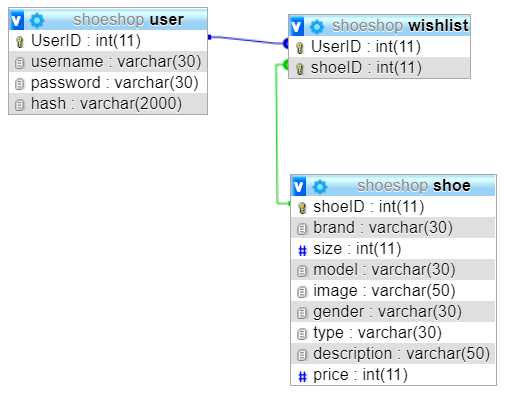
\includegraphics[width=1\textwidth]{db.png}
	\caption{Schema del database}
\end{figure}

\begin{center}
	\begin{tabular}{|l|l|l|}
		\hline
		\textbf{Nome Script}   &
		\textbf{Parametri GET} &
		\textbf{Descrizione}                                                                                           \\
		\hline
		add-cart               & id (scarpa)                                   & aggiunge scarpa al carrello           \\
		remove-cart            & id   (scarpa)                                 & rimuove scarpa da carrello            \\
		add-wishlist           & id                                            & aggiunge scarpa a id                  \\
		cart                   & nessuno                                       & JSON di tutte le scarpe nel carrello  \\
		category               & type, gender                                  & JSON delle scarpe corrispondenti      \\
		checklogin             & cookie                                        & logged se loggato NOT altrimenti      \\

		login                  & login / username password                     & logged
		se loggato not se input errato                                                                                 \\
		logout                 & nessuno                                       & termina la sessione e cancella cookie \\
		register               & \pbox{5cm}{jusernameRegister                                                          \\ passwordRegister}
		                       & \pbox{5cm}{Output: ok, username taken,error }                                         \\
		remove-cart            & id                                            & Rimuove scarpa dato id                \\
		remove-wishlist        & id                                            & Rimuove scarpa dato id                \\
		retrieve               & nessuno                                       & ritorna tutte le scarpe in JSON       \\
		session                & cookie, username                              &
		\pbox{5cm}{Controlla se la sessione è valida                                                                   \\
			Output: logged, not }                                                                                          \\
		single-retrieve        & id                                            & restituisce scarpa dato id in JSON    \\
		wishlist               & nessuno                                       & \pbox{5cm}{ritorna JSON delle scarpe
			\\ in wishlist utente} \\
		\hline
	\end{tabular}
\end{center}


\bigbreak
Le condizioni  di errore sono gestite in javascript a seconda dei
casi con un feedback all'utente

\end{document}